\documentclass[a4paper]{article}
\usepackage[utf8]{inputenc}
\usepackage[english]{babel}
\usepackage{amsmath} % per ambienti tipo cases
\usepackage{amssymb}
\usepackage{mathtools}
\usepackage{siunitx}
\usepackage{graphicx} % per includere figure
%\usepackage{subfigure}
\usepackage{wrapfig}
\usepackage{booktabs} % per le tabelle
\usepackage{caption}
\usepackage{fancyhdr}
\usepackage{hyperref}
\usepackage[section]{placeins}
\usepackage{microtype}
\usepackage{caption}
\usepackage{subcaption}
%\captionsetup[subfigure]{labelfont=rm}
\usepackage{verbatim} %multiline comments
\usepackage[backend=biber, style=numeric, safeinputenc, sorting=none]{biblatex}
\addbibresource{source.bib}	% uncomment for bibliography



%opening
\title{}
\author{}

\pagestyle{fancy}
\lhead{Musical Acoustics}
\chead{HL3}
\rhead{10743504, 10751919}
\newcommand{\Rarrow}{\mbox{\Large$\Rightarrow$}}

\begin{document}

\begin{titlepage}	
	\newcommand{\HRule}{\rule{\linewidth}{0.5mm}} % Defines a new command for horizontal lines, change thickness here
	
	\center % Centre everything on the page
	
	%------------------------------------------------
	%	Headings
	%------------------------------------------------
	
	
\includegraphics[width=.4\textwidth]{Logo_Politecnico_Milano.png}\\[0.4cm]
	\textsc{\LARGE}\\[0.3cm] % Main heading such as the name of your university/college
	
	\textsc{\large MSc. Music and Acoustic Engineering}\\[1cm] % Minor heading such as course title
	
	\textsc{\Large Musical Acoustics - A.Y. 2020/2021}\\[0.5cm] % Major heading such as course name
	
	%------------------------------------------------
	%	Title
	%------------------------------------------------
	
	\HRule\\[0.4cm]
	
	{\huge\bfseries HL3 – Modeling Techniques}\\[0.4cm] % Title of your document
	
	\HRule\\[1.5cm]
	
	
	
	{\large\textit{Authors' IDs:}}\\
	10743504, 10751919, % Your name
	%\\ \textsc{Gruppo 11}
	
	%------------------------------------------------
	%	Date
	%------------------------------------------------
	
	\vfill\vfill\vfill % Position the date 3/4 down the remaining page
	
	{\large\today} % Date, change the \today to a set date if you want to be precise
	
	%------------------------------------------------
	%	Logo
	%------------------------------------------------
	
	\vfill\vfill
	%\includegraphics[width=0.2\textwidth]{Politecnico_di_Milano.eps}\\[1cm] % Include a department/university logo - this will require the graphicx package
	
	%----------------------------------------------------------------------------------------
	
	\vfill % Push the date up 1/4 of the remaining page
	
	
\end{titlepage}

\section{Comments on the FD implementation}
The MATLAB code \verb|homework_piano.m| is able to perform a backward finite difference (FD) scheme which is used to simulate a piano string struck with a felt hammer. In the first part of the following report the numerical values chosen are illustrated while the second part describes briefly the actual FD algorithm. Finally the last section shows some results of such implementation.

\subsection{Simulation data}
  The string under consideration is tuned to C2 ($f_0 = \SI{52.8221}{\hertz}$). We chose a sampling frequency of $f_s = \SI{176.4}{\kilo\hertz}$ as suggested in \cite{saitis} and it's well above the Nyquist frequency so we don't expect aliasing in the time domain. Other dimensions that are not suggested in the assignment, such as string mass, hammer mass, string length etc. have been taken from \cite{saitis} and can be found listed in Tab. \ref{tab:vals} . The string has a linear mass $\mu = M_s / L$ and the tension applied on it at rest has been computed as $T_0 = 4L^2f_0^2\mu$ which determines that the speed of sound along the string is $c = \sqrt{T_0/\mu}$. The spatial sampling has been chosen under the limit imposed by the stability condition \cite{chaigne} $$ N_{max} = \sqrt{\frac{-1 + \sqrt{1 + 16 \epsilon \gamma ^2}}{8 \epsilon}} $$ where $\gamma = f_s / 2 f_0 $. The number of spatial steps has been set as $N = N_{max} -1 = 537$ and the relative spatial resolution is $X = \SI{0.0036}{\meter}$. 

 \begin{table}[h]
	\centering
	$\begin{array}{llc}
		\toprule
		\text{string length} &	L & \SI{1.92}{\meter}\\
		\text{string mass}   &	M_s & \SI{35e-3}{\kilogram}\\
		\text{string stiffness parameter} &	\epsilon & 7.5 	\times 10^{-6}\\
		\text{string stiffness coefficient} &	\kappa & 7.5 	\times 10^{-6}\\
		\text{relative striking position} &	a & 0.12 \\
		\midrule
		\text{viscous damping coefficient} & b_h & \SI{1e-4}{\second^{-1}}\\
		\text{hammer mass} & M_h & \SI{4.9e-3}{\kilogram} \\
		\text{hammer stiffness} &K & \SI{4e8}{\newton\per\meter}\\
		\text{stiffness exponent} &	p & 2.3 \\
		\midrule
		\text{hinge normalized impedance} &	\zeta_l & \SI{e20}{\second^3\meter^2\per\kilogram^2} \\
		\text{bridge normalized impedance} &	\zeta_b & \SI{e3}{\second^3\meter^2\per\kilogram^2} \\		
		\bottomrule
	\end{array}$
	\caption{Values considered in the simulation.}
	\label{tab:vals}
\end{table}

\subsection{FD algorithm}
The definition of temporal and spatial coordinate is the very first step of the FD implementation  
\begin{verbatim}
t = linspace(0, duration, tSamples); %temporal vector 
x = linspace( 1 , L , L/X  ); %spatial coordinate vector
\end{verbatim}

followed by the initialization of the string displacement $y(n,m)$, the hammer displacement (with respect to the contact point) $\eta(n)$, the hammer force $F(n)$ and the Hanning window $g(m)$, where $n \in t$ and $m \in x$. 

\begin{verbatim}
y = zeros(length(t), length(x)); %string displacement vector
eta = zeros(1 , length(t)); %hammer displacement vector
Fh = zeros(1 , length(t)); %hammer force vector
g = zeros(length(x), 1 ); %Hanning window vector
\end{verbatim}

At this point the Hanning window must be defined centred in the striking point $m_0$ and with a width of $2w$

\begin{verbatim}
m0 = ceil(x0/X); % hammer striking coordinate
wh = 0.1; %[m] half width of the hammer
w = ceil(wh/X); %sample of the hammer's width
gloc = hann(2*w); %local hanning window
g(m0-w:m0-w+length(gloc)-1)=gloc;
\end{verbatim}

and used to filter the force that is acting on the string $F(n,m) = F(n)g(m)$. At time $t=0$ ($n=1$) the string and the hammer are supposed to be still $y(1,m) = \eta(1) = 0$ and therefore the force $F(1) = 0$, since it is defined by the non-linear relation $F(n) = K|\eta(n) - y(n,m0)|^p$. The hammer displacement and the force at time $t= dt$ ($n=2$) is given by the velocity at time $t=0$, which is $Vh_0 = \SI{2.5}{\meter\per\second}$

\begin{verbatim}
eta(2) = Vh0*ts;
Fh(2) = K*(abs(eta(2) - y(2, m0)))^p;
\end{verbatim}

where $y(2,m_0)$ is assumed to be zero. After having defined the initial conditions, the backward FD loop can start by computing the displacement at time sample $n+1$ by knowing the displacement at $n$ and $n-1$.

 The scheme proposed below represents an implementation of the algorithm described in \cite{saitis}, where boundary conditions take into account the force transmission at the hinge and at the bridge, the displacement approximation at points just inside the domain ($x = dx$ and $x = L- dx$) and the hammer displacement at any time step. The FD formulas contain constant and convenient parameters which have not been mentioned before but can be found in \cite{saitis}.
 
 \begin{verbatim}
for n = 2:length(t)-1

Fh(n) = K*(abs(eta(n) - y(n, m0)))^p; % stricking force

for m = 1:length(x) %along the string

%forcing term definition at any time step

%if the hammer is no more in contact with the string
if(eta(n) < y(n, m0)) 
Fh(n) = 0;

else
F(n,m) = Fh(n)'*g(m); %windowed with the hanning
end

%boundary conditions
if(m==1) %if x = 0
y(n+1, m) = bl1*y(n, m) + bl2*y(n, m+1) + bl3*y(n, m +2) + ...
bl4*y(n-1, m) + blf*F(n,m);

elseif (m== length(x)) % if x = L
y(n+1, m) = br1*y(n, m) + br2*y(n, m-1) + br3*y(n, m -2) + ...
br4*y(n-1, m) + brf*F(n,m);

elseif( m ==length(x)-1 ) % if x = L - dx
y(n+1,m) = a1*(2*y(n, m+1) - y(n,m) + y(n,m-2)) + a2*(y(n,m+1) + ...
y(n,m-1)) + a3*y(n,m) + a4*y(n-1,m) + a5*(y(n-1,m+1) + y(n-1,m-1)) + ...
af*F(n,m);

elseif( m == 2) %if x = dx
y(n+1,m) = a1*(y(n, m +2) - y(n,m) + 2*y(n,m-1)) + a2*(y(n, m+1) ...
+ y(n,m-1)) + a3*y(n,m) + a4*y(n-1,m) + a5*(y(n-1,m+1) + ...
 y(n-1,m-1)) + af*F(n,m);

else 
%backward finite difference scheme "inside the domain"
y(n+1,m) = a1*(y(n, m+2) + y(n, m-2)) + a2*(y(n, m+1) +...
 y(n, m-1)) + ... a3*y(n,m) + a4*y(n-1,m) + ...
  a5*(y(n-1, m+1) + y(n-1,m-1)) + af*F(n,m);

end  
end

%hammer displacement approximation
eta(n+1) = d1*eta(n) + d2*eta(n-1) + df*Fh(n);   
end
 \end{verbatim}
 
 It can be noticed that the force $F(n)$ becomes zero when the hammer is no longer in contact with the string, so when $\eta(n) < y(n,m_0)$.
 
 \subsection{Time history and audio file}
 After the vector $y(n,m)$ has been computed for every value of $n$ and $m$ with the previous scheme, a visual representation can be obtained by plotting the displacement along $x$ for each time step. Actually, since in this way the animation would be too slow, it has been decided to plot $y(n,m)$ each $50$ time steps. A snapshot is shown in Fig. \ref{fig:displ} and an animation called \verb|string_displacement.gif| can be found attached to this report. 

Moreover, it has been computed a mean value of the displacement around the point $r_0 = L - m0$ (see Fig.\ref{fig:historyone} and Fig.\ref{fig:historytwo} ) by taking averaging 12 spatial samples: 6 on the left of $r_0$ and 6 on the right of $r_0$

\begin{verbatim}
r0 = ceil((L-x0)/X); %coordinate of the striking specular point
yspec = [y(:,r0+1)' ; y(:,r0+2)'; y(:,r0+3)'; y(:,r0+4)'; ...
 y(:,r0+5)'; y(:,r0+6)'; y(:,r0-1)'; y(:,r0-2)'; ...
 y(:,r0-3)'; y(:,r0-4)'; y(:,r0-5)'; y(:,r0-6)'];
yaudio = mean(yspec);
\end{verbatim}

from which the vector \verb|yaudio| has been gained by a factor of $\times 100$ in order to make it audible, then converted into a sound and stored it.

\begin{verbatim}
sound(100*yaudio, fs); %Play the sound
 filename = '10751919_Lercari_10743504_Lampis_piano.wav';
audiowrite(filename, 100*yaudio,fs); 
\end{verbatim}

 \begin{figure}[h]
	\centering
	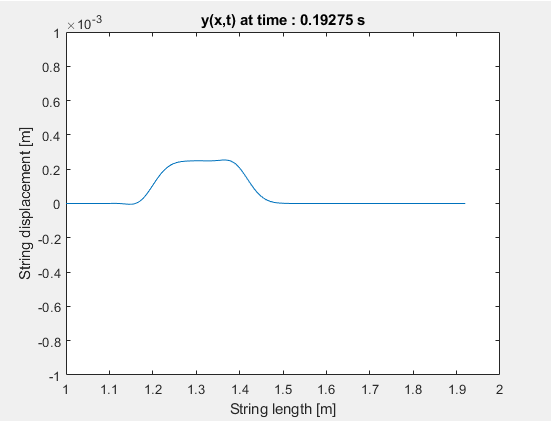
\includegraphics[width=0.75\linewidth]{displacement.png}
	\caption{Snapshot from string displacement animation.}
	\label{fig:displ}
\end{figure}

 \begin{figure}[h]
	\centering
	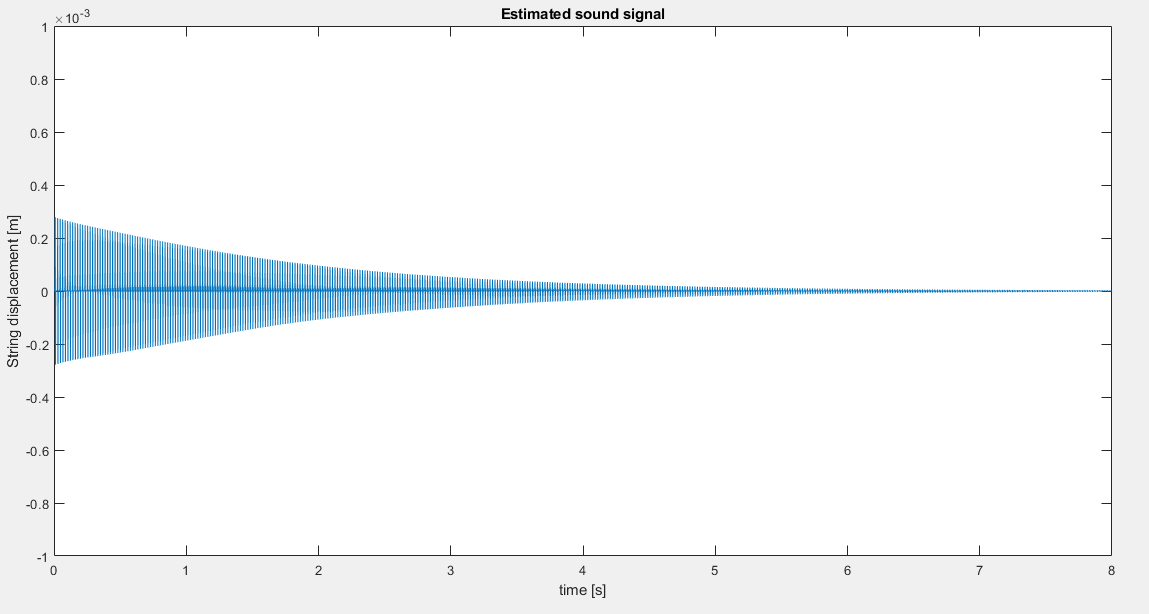
\includegraphics[width=0.75\linewidth]{sound_two.png}
	\caption{Time history of the mean of the string displacement.}
	\label{fig:historyone}
\end{figure}

 \begin{figure}[h]
	\centering
	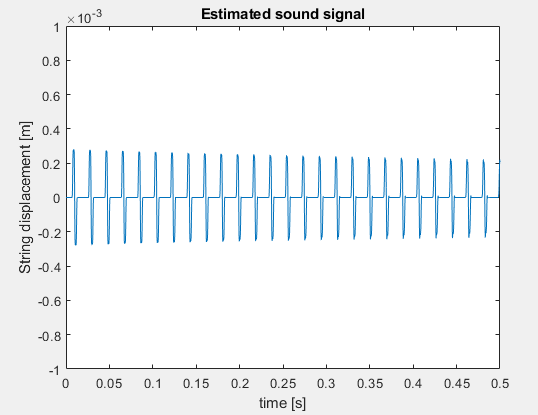
\includegraphics[width=0.75\linewidth]{sound_one.png}
	\caption{Time history of the mean of the string displacement during the first 500 ms.}
	\label{fig:historytwo}
\end{figure}

\section{Modeling a guitar with an electrical analog}
\subsection{Circuit for the body}

\begin{figure}[h!]
	\centering
	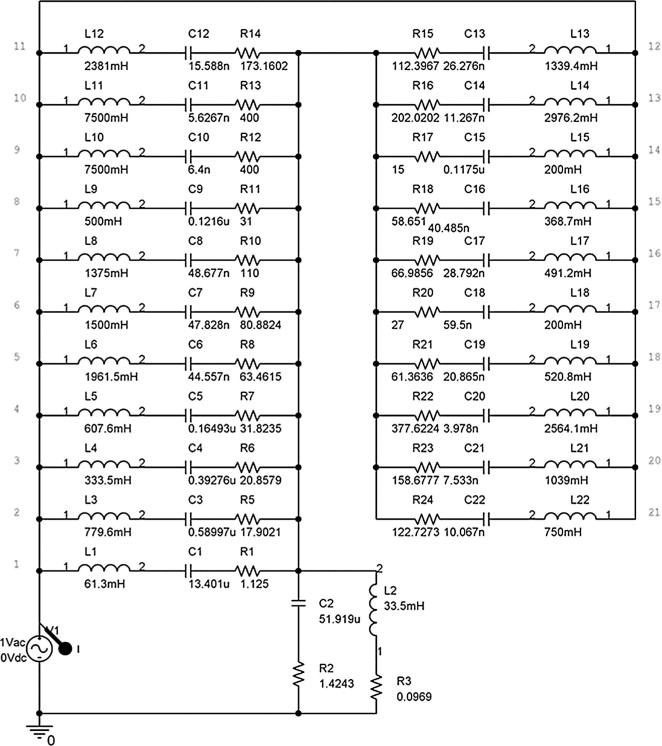
\includegraphics[width=0.5\linewidth]{guitar_body.jpg}
	\caption{Network analog of the guitar body, constructed by expanding on the two-mass model.}
	\label{fig:body}
\end{figure}

The simplest model of the body of a guitar is the two-mass model, which corresponds to the circuit in Fig. \ref{fig:body} when only the first of the many RLC series is present. This is a lumped parameter model which accounts well for the lowest modes of the guitar body. If we want to include higher modes in the model using theoretical arguments, we are going to need some kind of distibuted-parameter component, at least for the top plate. Alternatively, we can follow an empirical approach such as the one presented in \cite{leefrench}. Here, 20 additional resonances of the top plate are modelled as RLC series in parallel with the first one, expanding on the two-mass model. The components are then tuned to make the circuit response resemble that of an actual instrument (as measured by the authors). 
\begin{wrapfigure}{r}{0.4\textwidth}
	\centering
	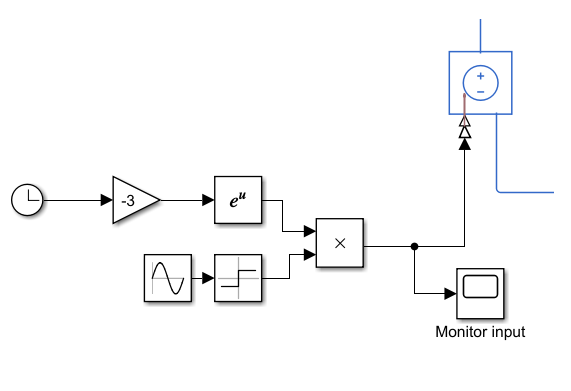
\includegraphics[width=0.98\linewidth]{inputModel.png}
	\caption{Simplified model for the input signal at the bridge.}
	\label{fig:dampsquare}
\end{wrapfigure}
This approach allows us to use a representation based only on discrete, passive components, simplifying the implementation significantly and granting us the possibility of using one of the many available tools for the simulation of analog electrical networks. In particular, the implementation we present in this section has been done with Simscape.


In the first part of the implementation we are concerned with designing the body circuit. Here we run a simulation ignoring, for the moment, the modeling of the string: to do so we use a rough approximation for the string signal, given by a damped square wave (Fig. \ref{fig:dampsquare}). The body network was constructed using the component values shown in Fig. \ref{fig:body} and it can be found in \texttt{exercise\_6a.slx}. The resulting signal can be seen in Fig. \ref{fig:nostring}, and it has been saved as an audio file in \texttt{simplifiedInput.wav}.

\begin{figure}[h]
	\centering
	\begin{subfigure}{0.4\linewidth}
		\centering
		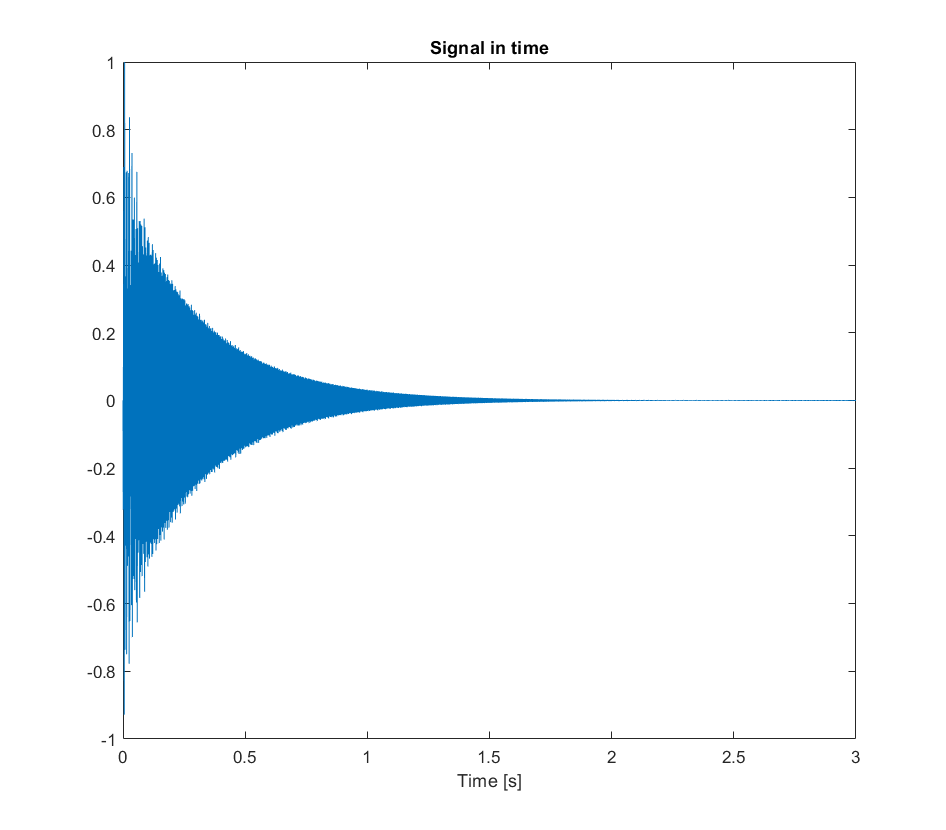
\includegraphics[width=0.9\linewidth]{simpOut.png}
	\end{subfigure}
~
	\begin{subfigure}{0.4\linewidth}
		\centering
		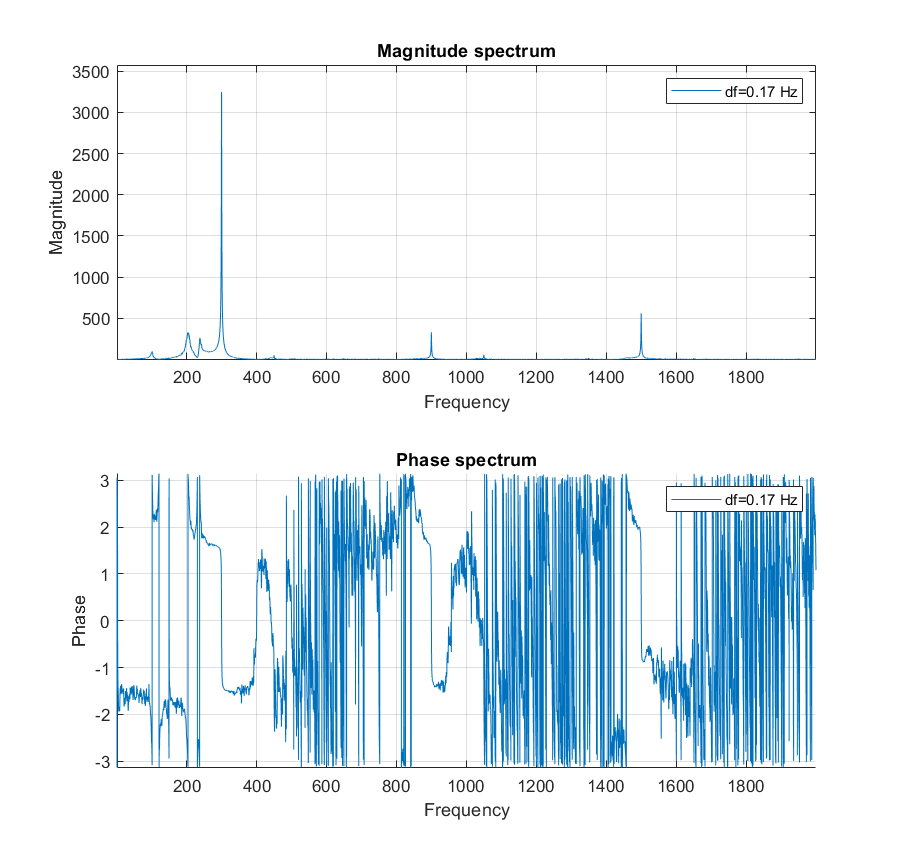
\includegraphics[width=0.9\linewidth]{simpSpect.png}
	\end{subfigure}
	\caption{Time history and FFT of the (normalized) sound with the simplified input.}
	\label{fig:nostring}
\end{figure}


\subsection{Circuit for the string (and the whole guitar)}
\begin{figure}[h]
	\centering
	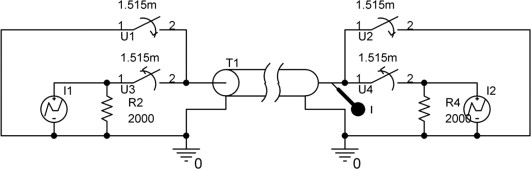
\includegraphics[width=0.7\linewidth]{guitar_string.jpg}
	\caption{Electrical analog of a guitar string.}
	\label{fig:guitarstring}
\end{figure}

The second part of the implementation involves instead the modeling of the string. The string itself can be represented by a transmission line, with the ideal reflections at the ends corresponding to short circuits. In parallel with the short circuits, we can see at both ends a current generator with a load impedance, used to model the plucking of the string. The generators provide the initial conditions by feeding triangular inputs to the transmission line. After half a period of the fundamental, the generator switches open and the short-circuit switches close, leaving the signal to reflect back and forth on the transmission line.

The string circuit is connected to the body circuit at the U2 switch (Fig. \ref{fig:guitarstring}. The sound is recovered by taking the time derivative (approximated with finite differences) of the current at this point, which can be shown to be proportional to the vertical force at the bridge.  The resulting signal can be seen in Fig. \ref{fig:complete} and it has been saved as an audio file in \texttt{completeGuitar.wav}. The MATLAB script that executes the simulation is \texttt{exercise6\_script.m}, while the complete circuit model can be found in \texttt{exercise\_6.slx}. The result is a much better approximation of the sound of a guitar than the two-mass system, and this is especially apparent in how the fast plucking transient sounds, as a consequence of the more realistic response in the higher frequency range.

\begin{figure}[h]
	\centering
	\begin{subfigure}{0.48\linewidth}
		\centering
		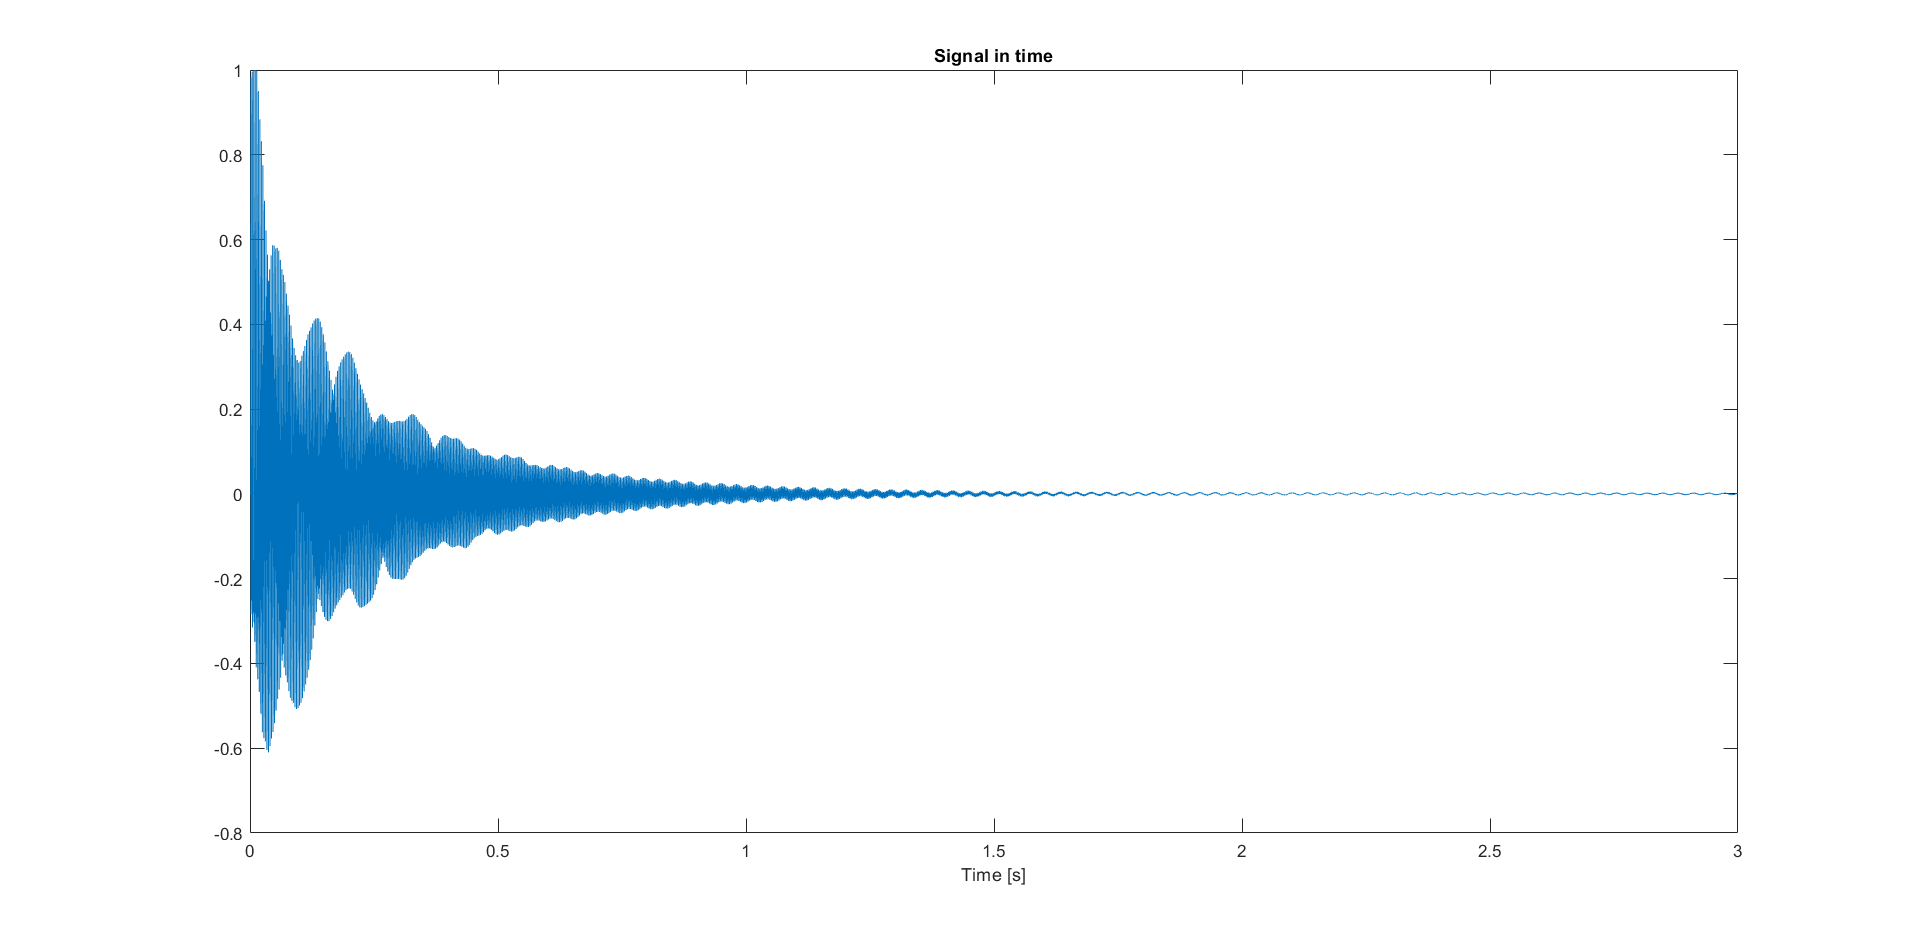
\includegraphics[width=0.95\linewidth]{pluck.png}
	\end{subfigure}
	~
	\begin{subfigure}{0.48\linewidth}
		\centering
		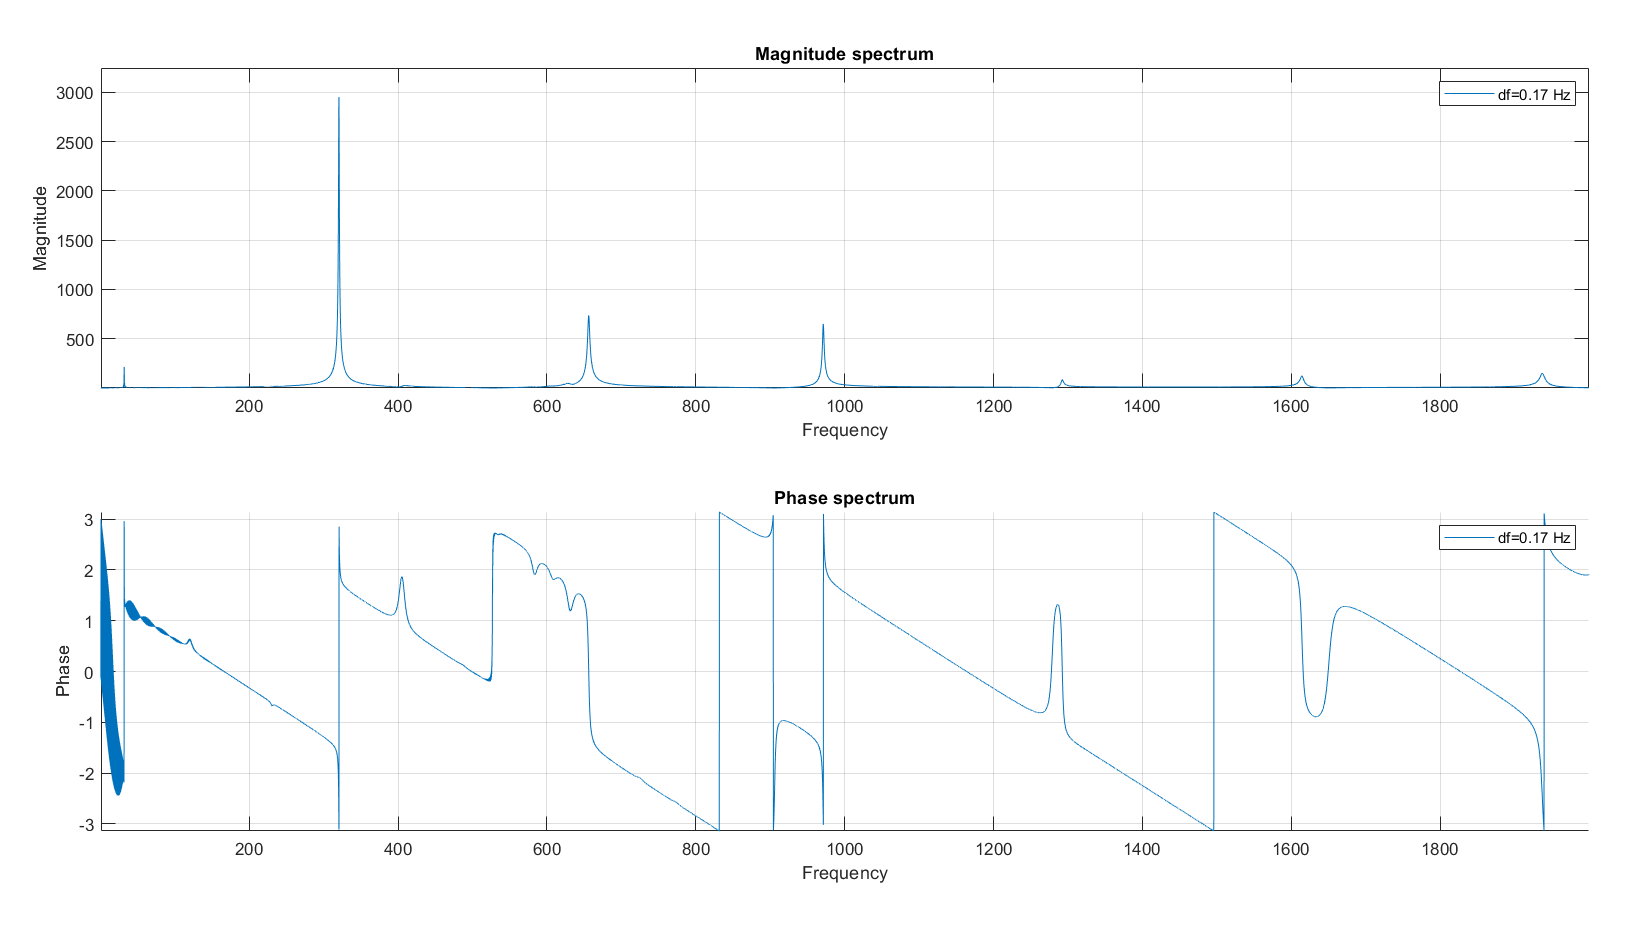
\includegraphics[width=0.95\linewidth]{guitSpectrum.png}
	\end{subfigure}
	\caption{Time history and FFT of the (normalized) sound produced by the complete guitar simulation.}
	\label{fig:complete}
\end{figure}


\printbibliography


\end{document}